\section[Background]{Background on {\em Drosophila} imaging}

\begin{frame}{Importance of Symmetries in Reconstructing Dynamics}

{\bf Goal:} Construct a smooth trajectory from snapshots \footcite{kemelmacher2011exploring}

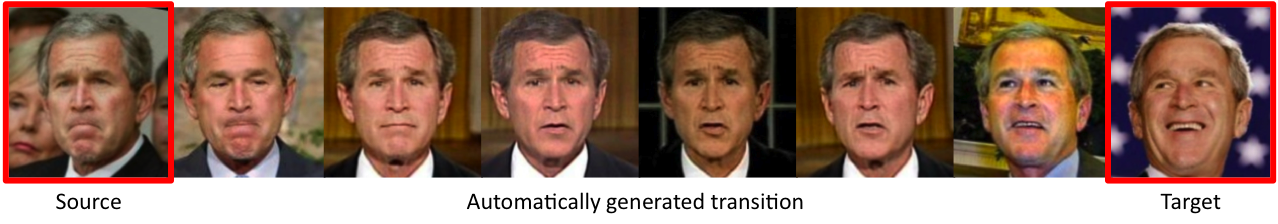
\includegraphics[width=\textwidth]{photobios}

However, these snapshots can be taken from different viewing angles and rotations, and so we must {\em factor out} the relevant symmetries before constructing a representative trajectory

We will look at snapshots of {\em Drosophila} throughout development and try to construct a smooth, representative trajectory of the developmental dynamics

\end{frame}

\begin{frame}{Imaging Dorsoventral Patterns in {\em Drosophila} \footcite{chung2010microfluidic}}

	\centering
    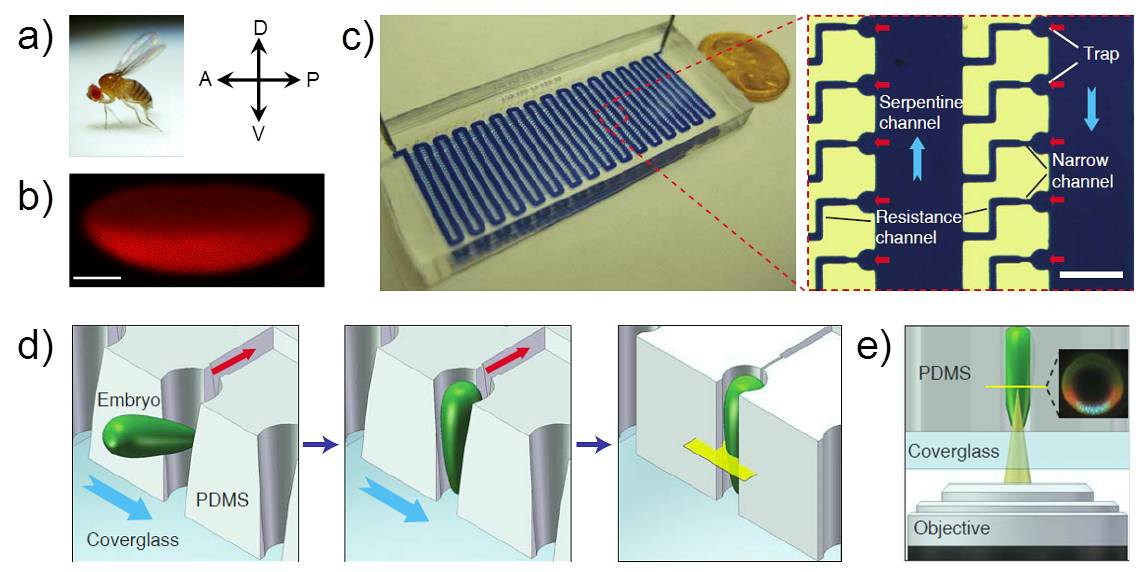
\includegraphics[width=0.75\textwidth]{drosophila_imaging_setup}
    
	\begin{itemize}
        \item We can easily obtain snapshots many embryos using a high--throughput microfluidic device
        \item Each embryo is fixed at a slightly different developmental time (``cross-sectional data'')
        \item We would like to order the data from multiple embryos in time that we can reconstruct the developmental dynamics in {\em Drosophila}
    \end{itemize}
\end{frame}


\begin{frame}{ERK Activation in {\em Drosophila}}

	We would like to reconstruct the spatiotemporal dynamics \\
	of the activation of the ERK pathway in {\em Drosophila} embryos\\
	during nuclear cycle 14 (the third hour of development)

    \centering
	\begin{minipage}{0.3\textwidth}
	    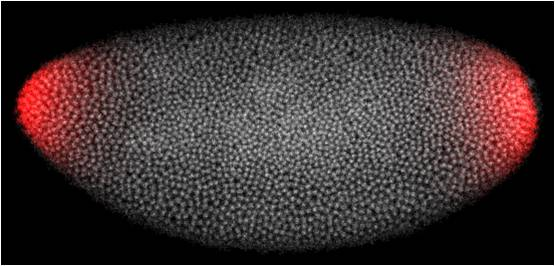
\includegraphics[width=\textwidth]{erk_10min}\\
	    {\scriptsize \em 10 minutes \par}
	\end{minipage}
	\begin{minipage}{0.3\textwidth}
	    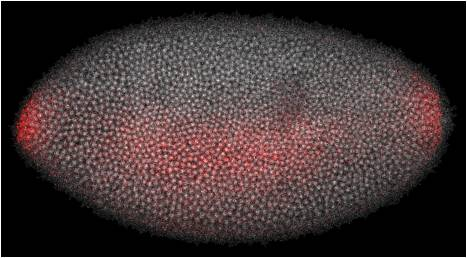
\includegraphics[width=\textwidth]{erk_25min}\\
	    {\scriptsize \em 25 minutes \par}
	\end{minipage}
	\begin{minipage}{0.3\textwidth}
	    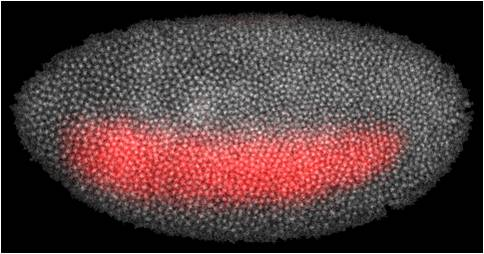
\includegraphics[width=\textwidth]{erk_45min}\\
	    {\scriptsize \em 45 minutes \par}
	\end{minipage}
	
	\begin{itemize}
		\item We measure the activation of ERK by staining embryos for double-phosphorylated ERK (dpERK); ERK is double-phosphorylated  directly downstream of the ERK pathway, and so the presence of dpERK indicates activation of the ERK pathway
	
		\item However, we cannot fluorescently tag ERK within the developing embryo because we are interested in a specific phosphorylation state of the molecule
		
		\item Instead, we must {\em fix} the embryo and then use an antibody stain for dpERK
	
		\item Therefore, we cannot obtain live images of the evolution of dpERK in {\em Drosophila} embryos
	\end{itemize}
	
\end{frame}




%\begin{frame}{Motivation: How Do Cells Obtain Unique Functions?}
%
%    \begin{tikzpicture}
%        \node (embryo1) {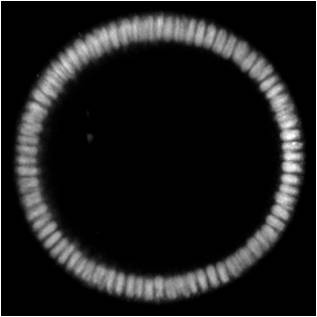
\includegraphics[width=0.15\textwidth]{embryo_bw}};
%        \draw[gray,<->] (embryo1.south west) --  (embryo1.south east) node[below,midway] { \tiny $100 \mu m$};
%        
%        \node[below=0.1in of embryo1, text width=0.15\textwidth, align=center] (text1)  {{\scriptsize Cells}};
%		
%		\node[right=0.3in of embryo1] (embryo3)  {     
%        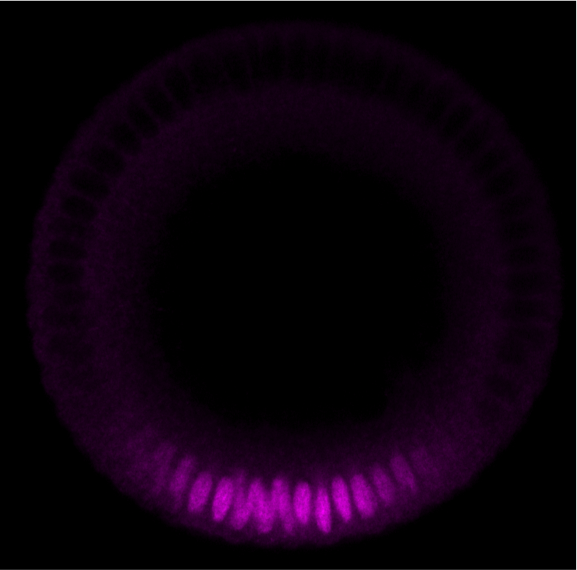
\includegraphics[width=0.2\textwidth]{dorsal}} edge[<-] (embryo1);
%        \draw[gray, <->] (embryo3.south west) --  (embryo3.south east) node[below,midway] { \tiny $100 \mu m$};
%        \node[below=0.1in of embryo3, text width=0.15\textwidth, align=center] (text2)  {{\scriptsize Morphogens diffuse \footnotemark \par}};
%		\node[above=0in of embryo3] (flag)  {     
%        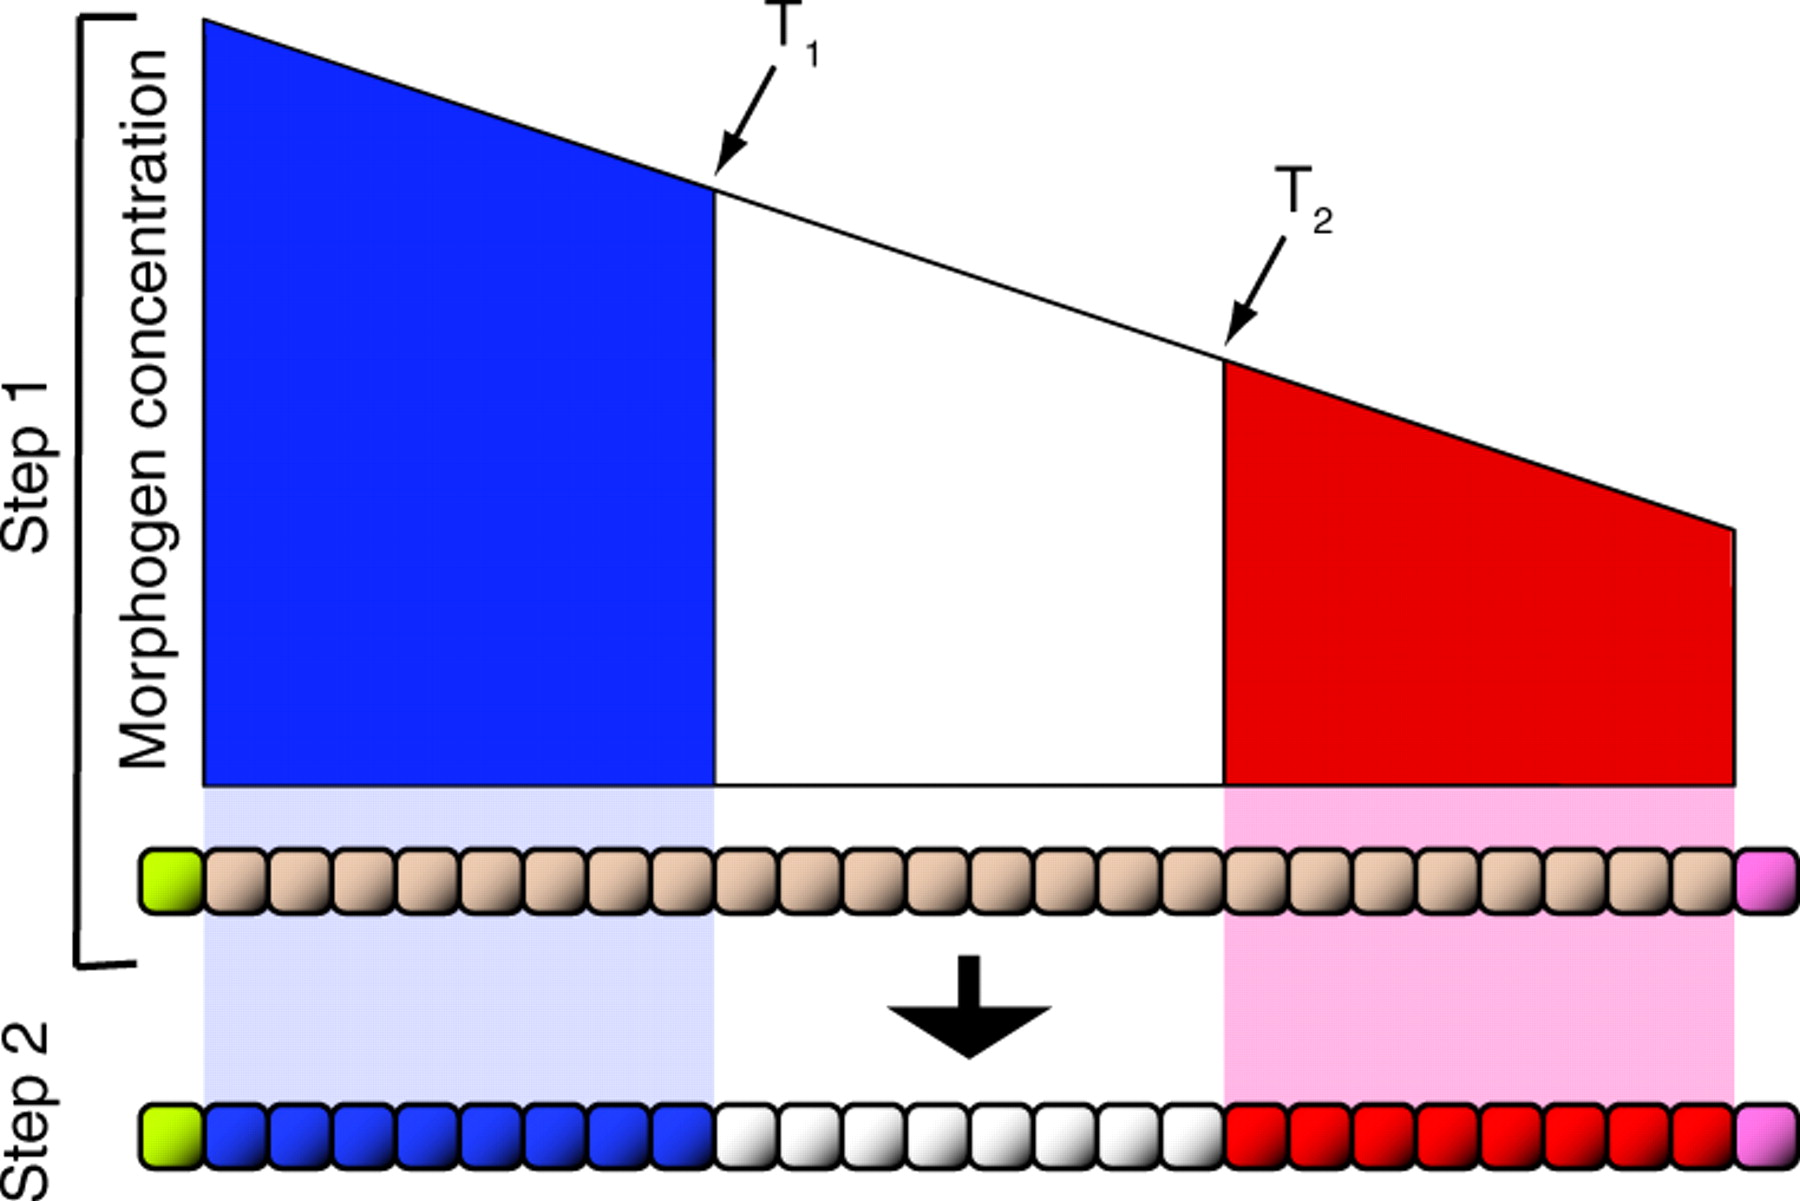
\includegraphics[width=0.2\textwidth]{french_flag}};
%        
%        \node[right=0.3in of embryo3] (embryo2)  {     
%        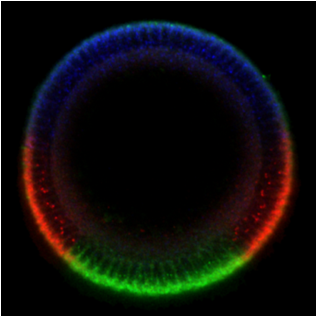
\includegraphics[width=0.15\textwidth]{embryo_color}} edge[<-] (embryo3);
%                \draw[gray,<->] (embryo2.south west) --  (embryo2.south east) node[below,midway] { \tiny $100 \mu m$};
%
%        \node[below=0.1in of embryo2, text width=0.15\textwidth, align=center] (text2)  {{\scriptsize Different proteins are produced in different regions \par}};
%
%        \node[right=0.3in of embryo2] (nervous)  {
\includegraphics[width=0.15\textwidth]{nervous_system}} edge[<-] (embryo2);
%
%        \node[above=0.1in of nervous] (skin)  {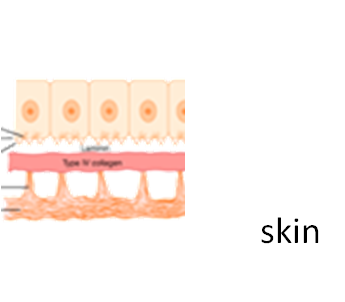
\includegraphics[width=0.15\textwidth]{skin}} edge[<-] (embryo2);
%
%        \node[below=0.1in of nervous] (muscle)  {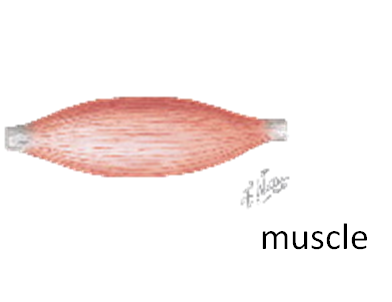
\includegraphics[width=0.15\textwidth]{muscle}} edge[<-] (embryo2);
%    \end{tikzpicture}
%
%	\footcitetext{jaeger2008regulative}
%	
%	{\small Different pathways are {\em activated} in different areas of the organism,  
%	leading to the production of different proteins and different cells developing~different~functions \par}
%
%\end{frame}
%
%\begin{frame}{ERK Activation Across Species}
%	\begin{itemize}
%		\item 	Extracellular signal-regulated kinases (ERKs) are singalling proteins that regulate mitosis and meiosis in cells.
%
%		\item	ERK activation is conserved among many species.
%
%	\end{itemize}
%	
%    \centering
%    \begin{minipage}{0.2\textwidth}
%        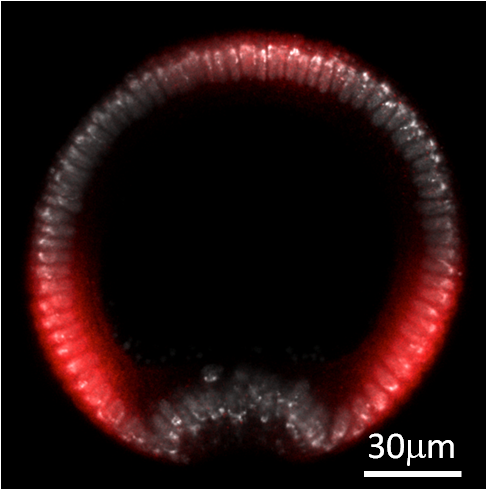
\includegraphics[width=\textwidth]{drosophila_erk}\\
%        {\scriptsize \em Drosophila \par}
%    \end{minipage}
%    \hspace{0.5in}
%    \begin{minipage}{0.2\textwidth}
%        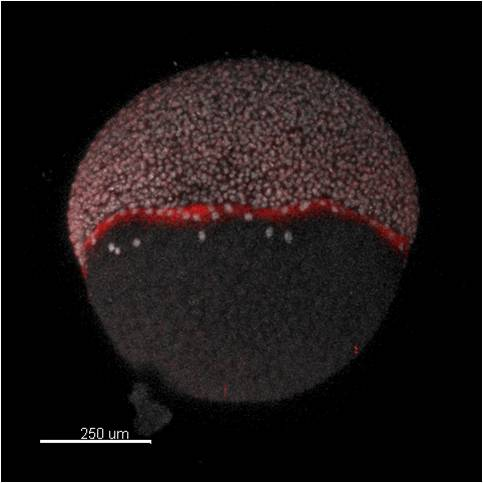
\includegraphics[width=\textwidth]{zebrafish_erk}\\
%        {\scriptsize \em zebrafish \par}
%    \end{minipage}
%    \vspace{0.2in}
%    
%    \centering
%    \begin{minipage}{0.4\textwidth}
%        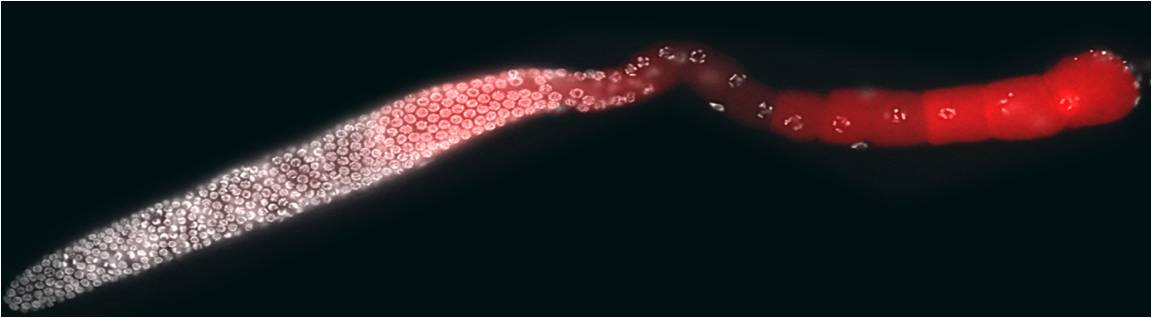
\includegraphics[width=\textwidth]{celegans_erk}\\
%        {\scriptsize \em C. elegans \par}
%    \end{minipage}
%    
%	\vspace{0.1in}
%    ERK stained (in red) in several model organisms.
%    
%\end{frame}





\begin{frame}{Measuring Developmental Time from Membrane Markers}

	\centering
    The current standard practice is to use membrane thickness \\to measure the age of an embryo \footcite{lim2013kinetics, lecuit2002slam}\\
    \vspace{0.2in}
    \begin{tikzpicture}
        \node (dpERK_5min) {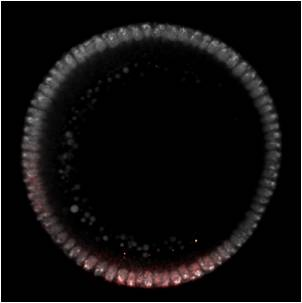
\includegraphics[width=0.1\textwidth]{dpERK_5min}};
        \node[right=0in of dpERK_5min] (mem_5min) {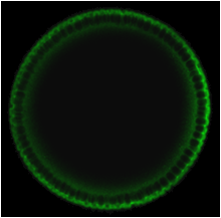
\includegraphics[width=0.1\textwidth]{membrane_5min}};
        \node[below=0.1in of dpERK_5min] (dpERK_20min) {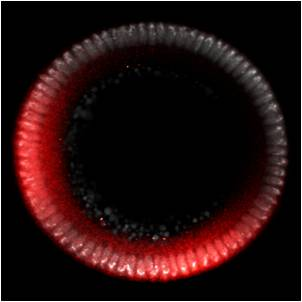
\includegraphics[width=0.1\textwidth]{dpERK_20min}};
        \node[right=0in of dpERK_20min] (mem_20min) {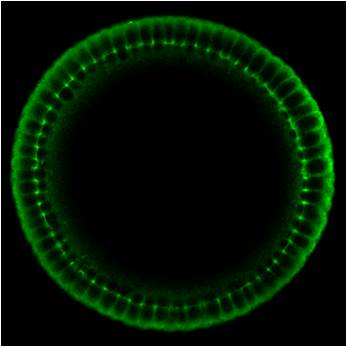
\includegraphics[width=0.1\textwidth]{membrane_20min}};
        \node[below=0.1in of dpERK_20min] (dpERK_45min) {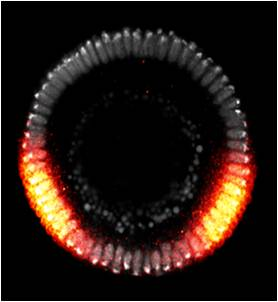
\includegraphics[width=0.1\textwidth]{dpERK_45min}};
        \node[right=0in of dpERK_45min] (mem_45min) {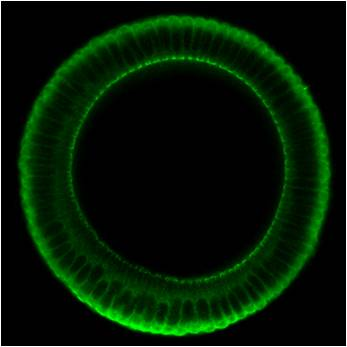
\includegraphics[width=0.1\textwidth]{membrane_45min}};
        \node[right=0.5in of mem_20min] (calibration) {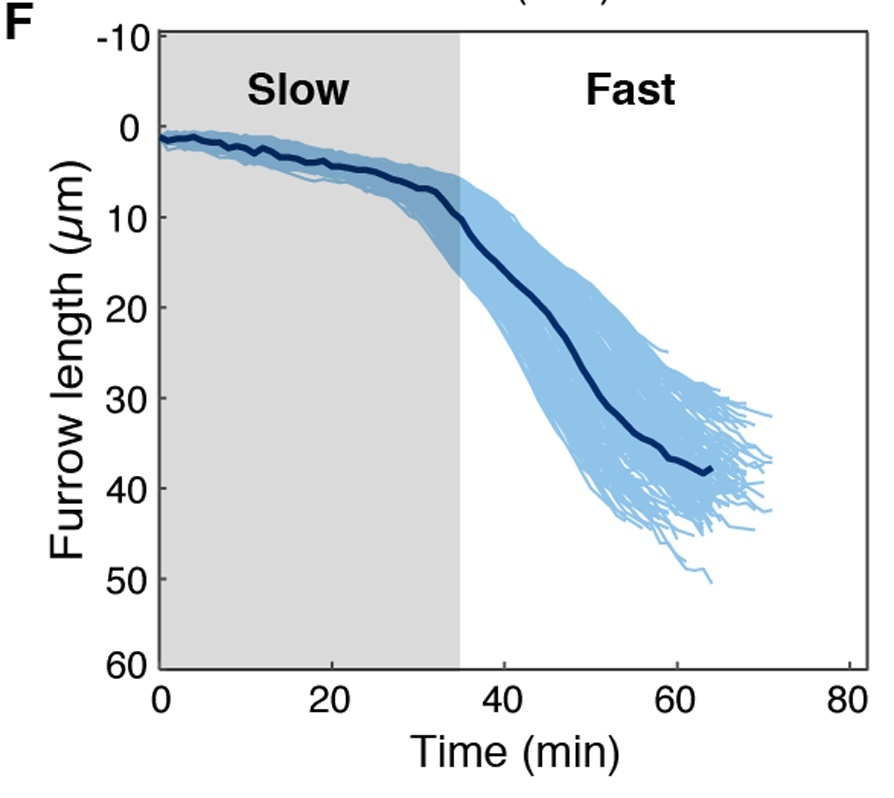
\includegraphics[width=0.3\textwidth]{calibration_curve}} edge[<-] (mem_5min) edge[<-] (mem_20min) edge[<-] (mem_45min);
        \node[right=2.5in of mem_20min] (time_20) {20 minutes} edge[<-] (calibration);
        \node[right=2.5in of mem_5min] (time_5) {5 minutes} edge[<-] (calibration);
        \node[right=2.5in of mem_45min] (time_45) {45 minutes} edge[<-] (calibration);
    \end{tikzpicture}

\end{frame}

\begin{frame}{Reconstructing Dynamics from Snapshots}

	\begin{tikzpicture}
		\node (schematic) {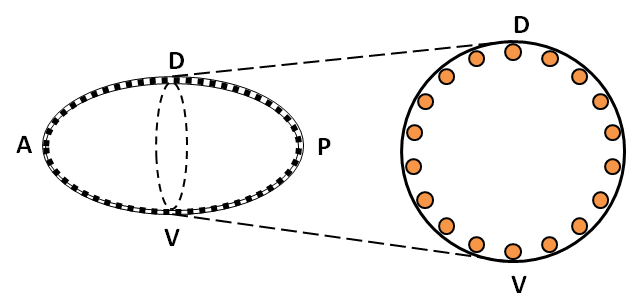
\includegraphics[width=0.25\textwidth]{drosophila_schematic}};
		\node [below=0in of schematic, text width=0.2\textwidth, align=center] (text1) {{\scriptsize Schematic of {\em Drosophila} embryo \\ (longitudinal and cross-section) \par}};

		\node [right=0.2in of schematic] (dpERK_image) {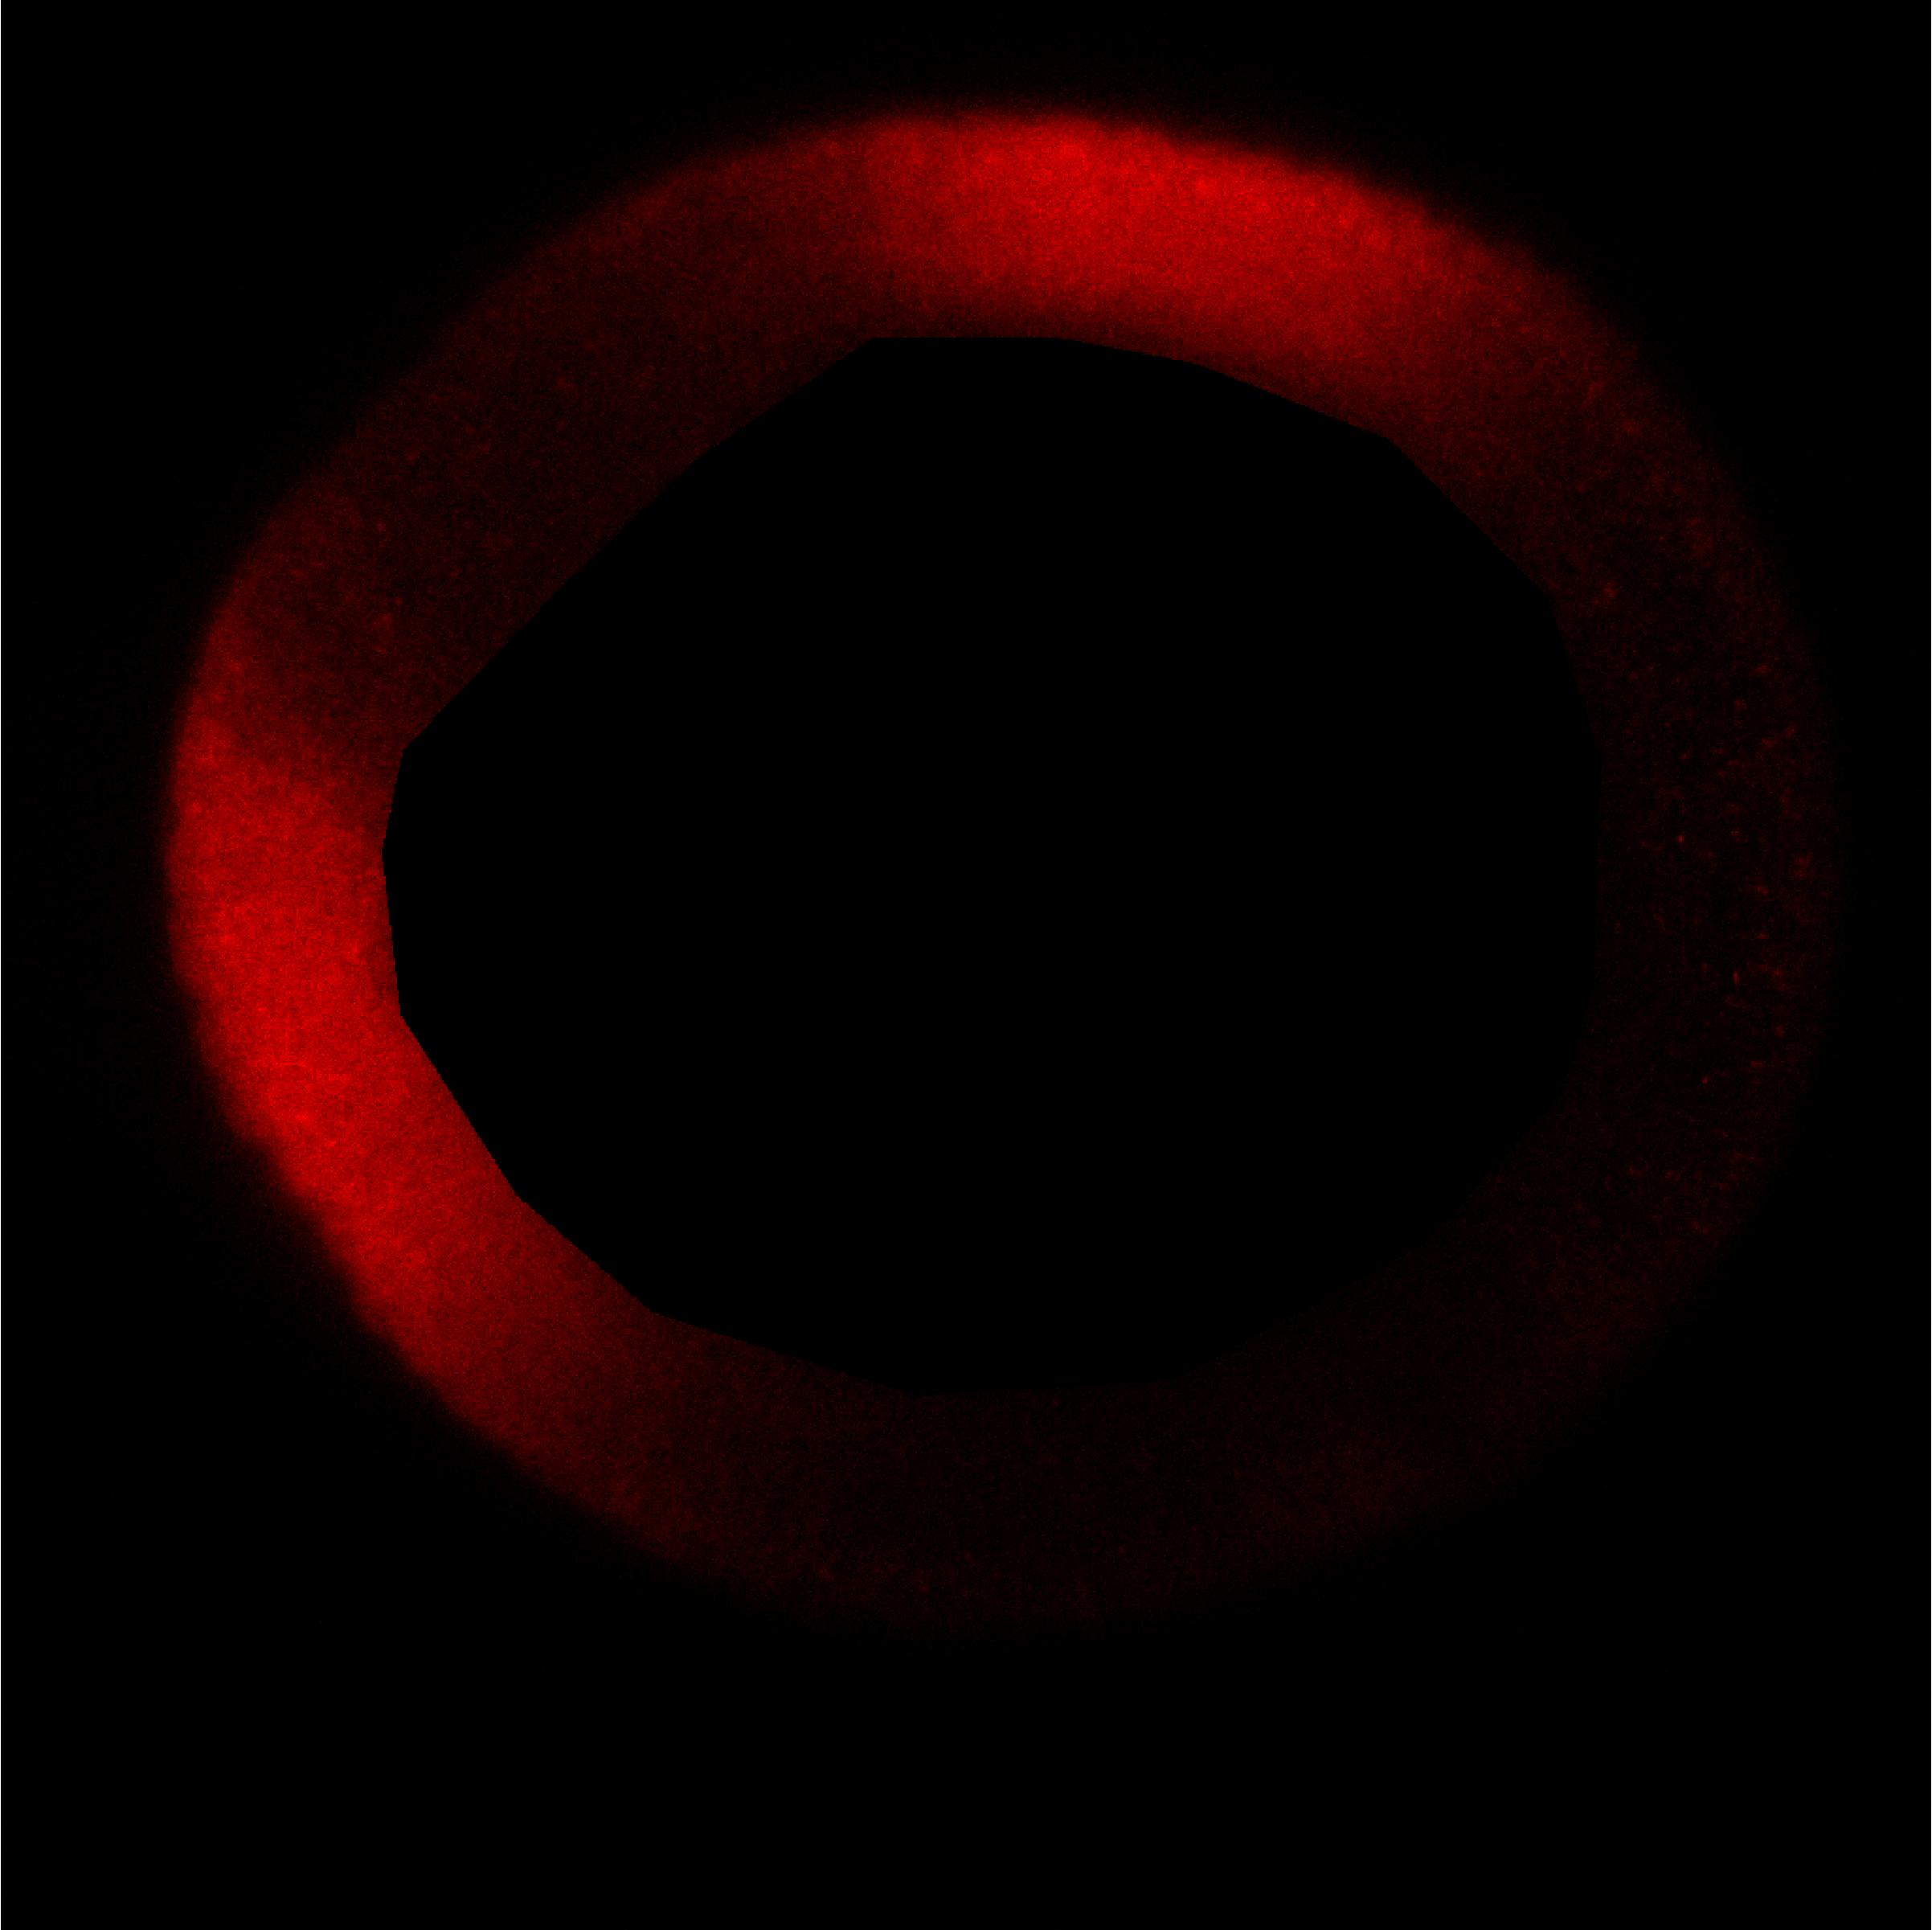
\includegraphics[width=0.15\textwidth]{drosophila_dpERK}} edge[<-] (schematic);
		\draw[gray,<->] (dpERK_image.south west) --  (dpERK_image.south east) node[below,midway] { \tiny $100 \mu m$};
		\node [below=0.1in of dpERK_image, text width=0.2\textwidth, align=center] (text1) {{\scriptsize Embryo cross-section fluorescently stained for the protein dpERK \par}};
		
		\node [right=0.2in of dpERK_image] (dpERK_circle) {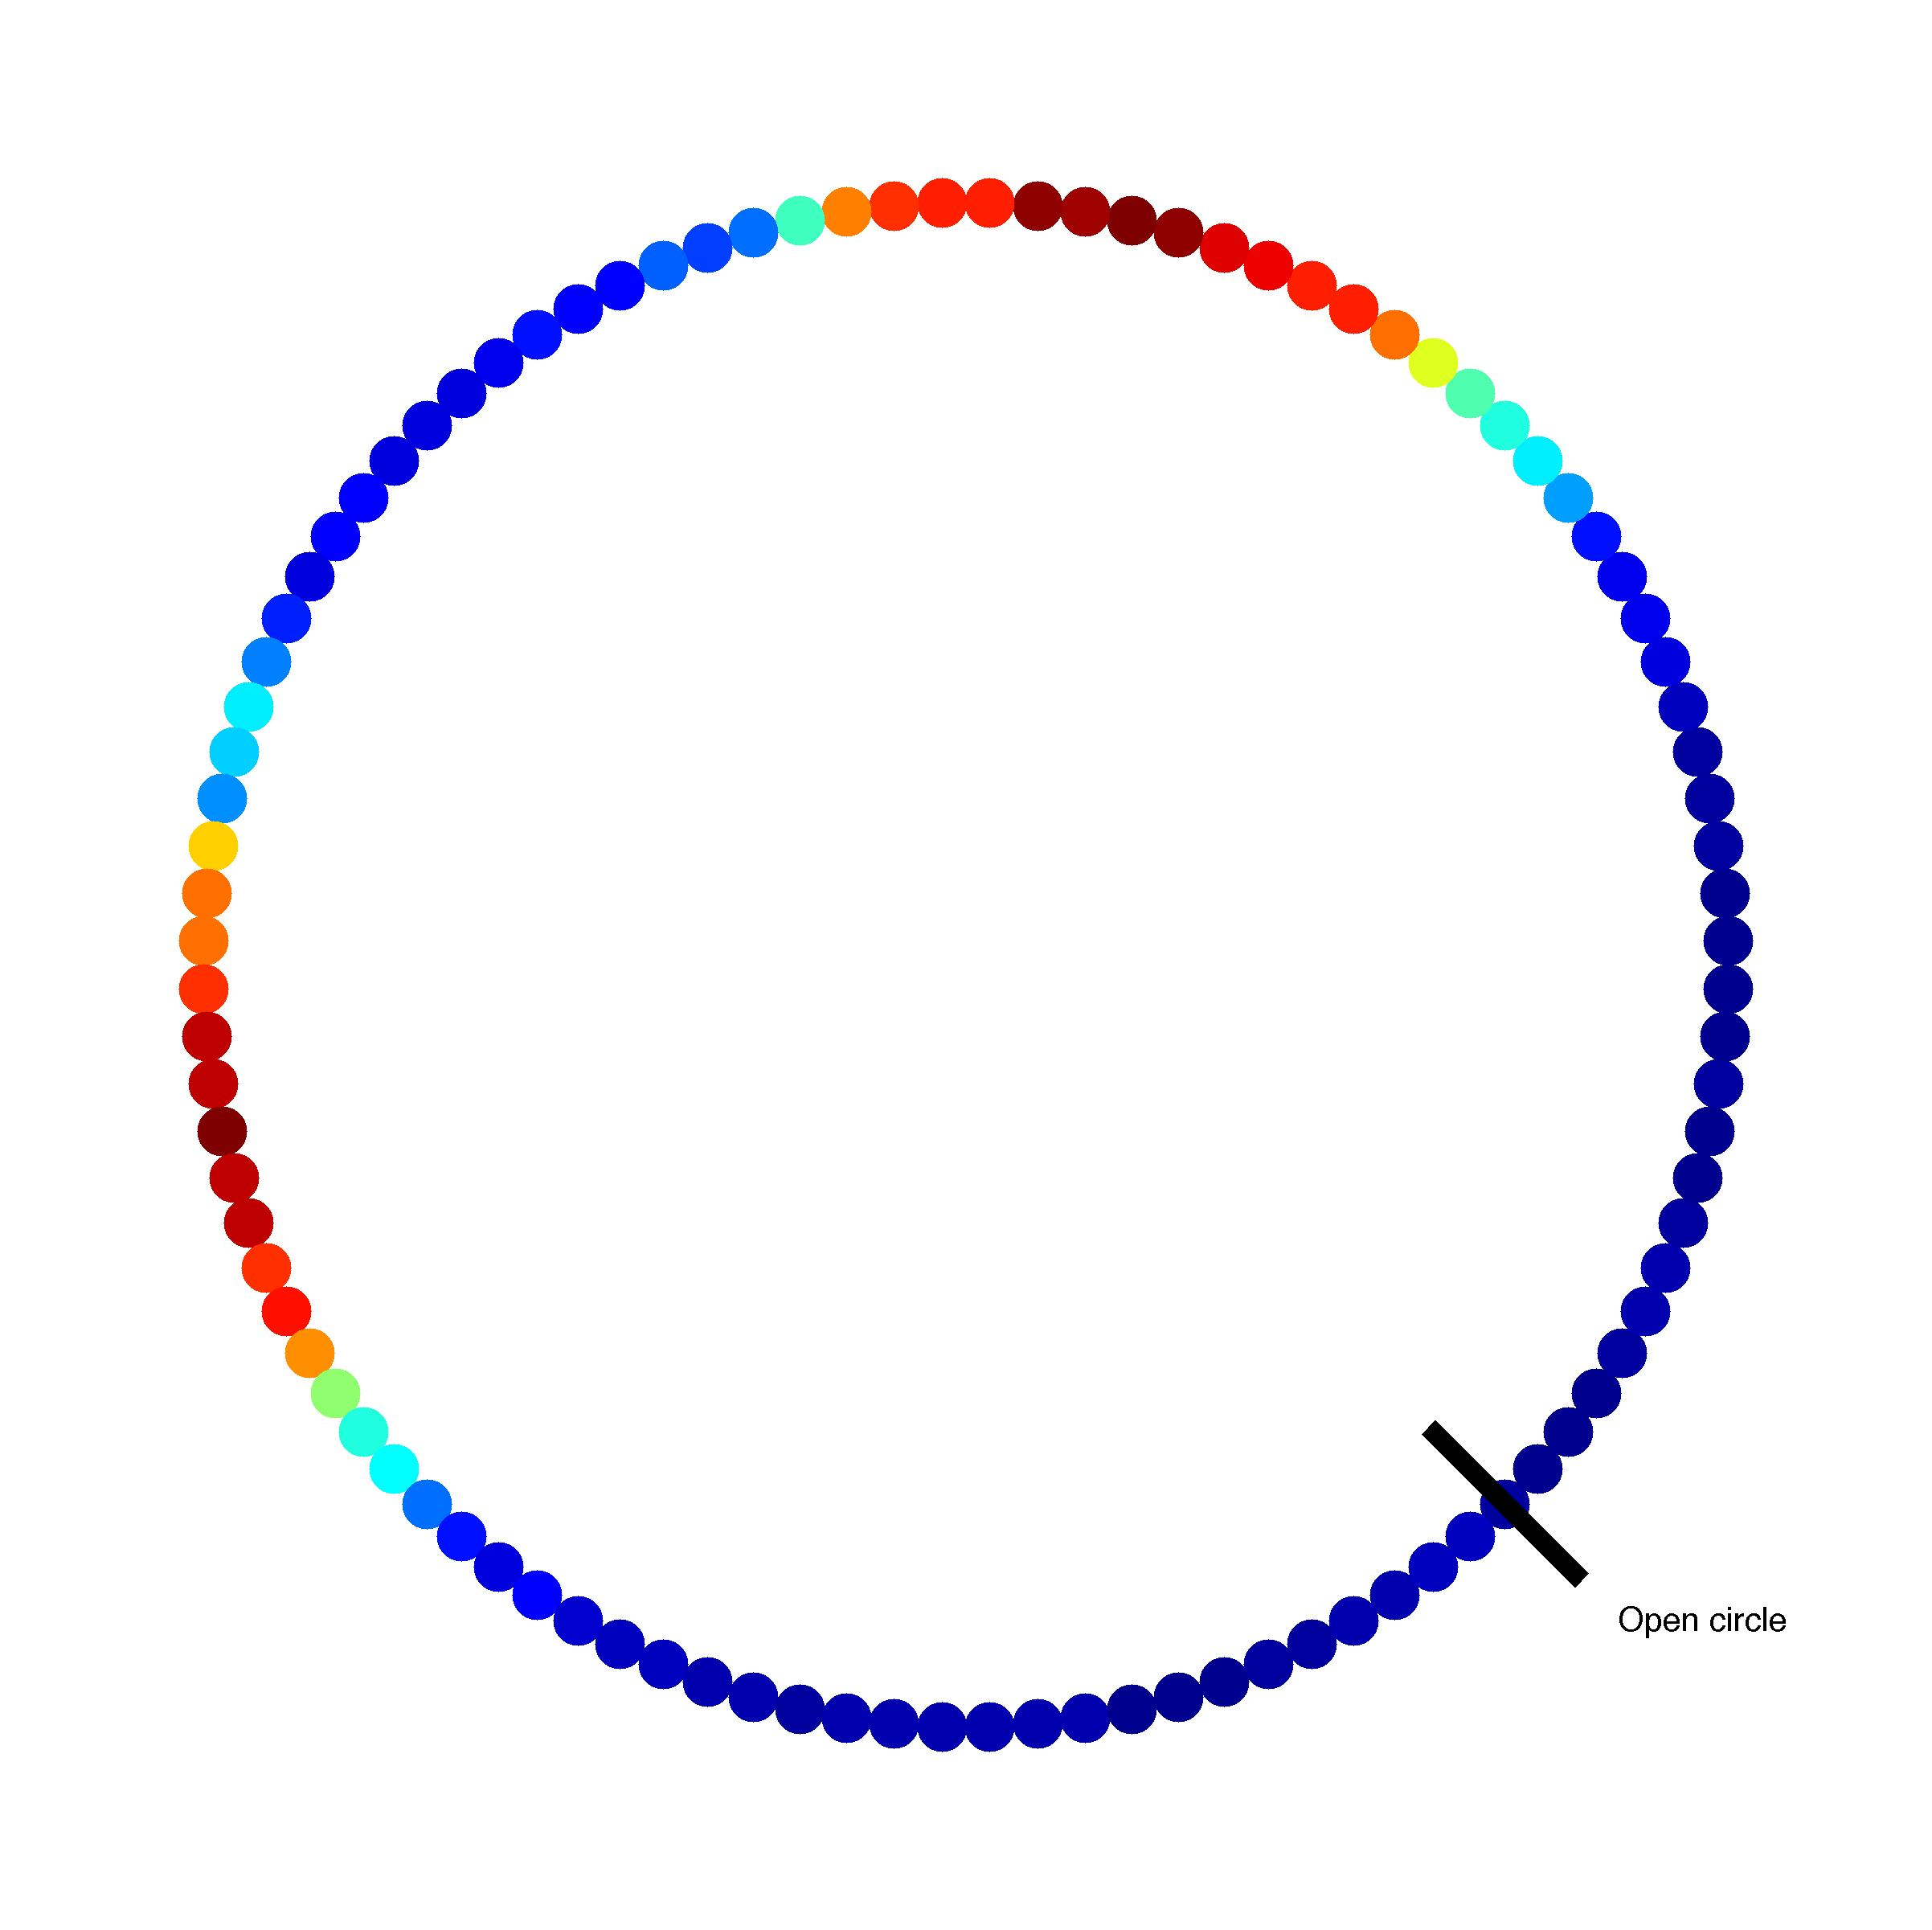
\includegraphics[width=0.15\textwidth]{circle_profile.jpg}} edge[<-] (dpERK_image);
		\node [below=0in of dpERK_circle, text width=0.2\textwidth, align=center] (text1) {{\scriptsize Fluorescent staining is converted to intensity of dpERK around the circumference of the embryo \par}};
		
		\node [right=0.2in of dpERK_circle] (dpERK_line) {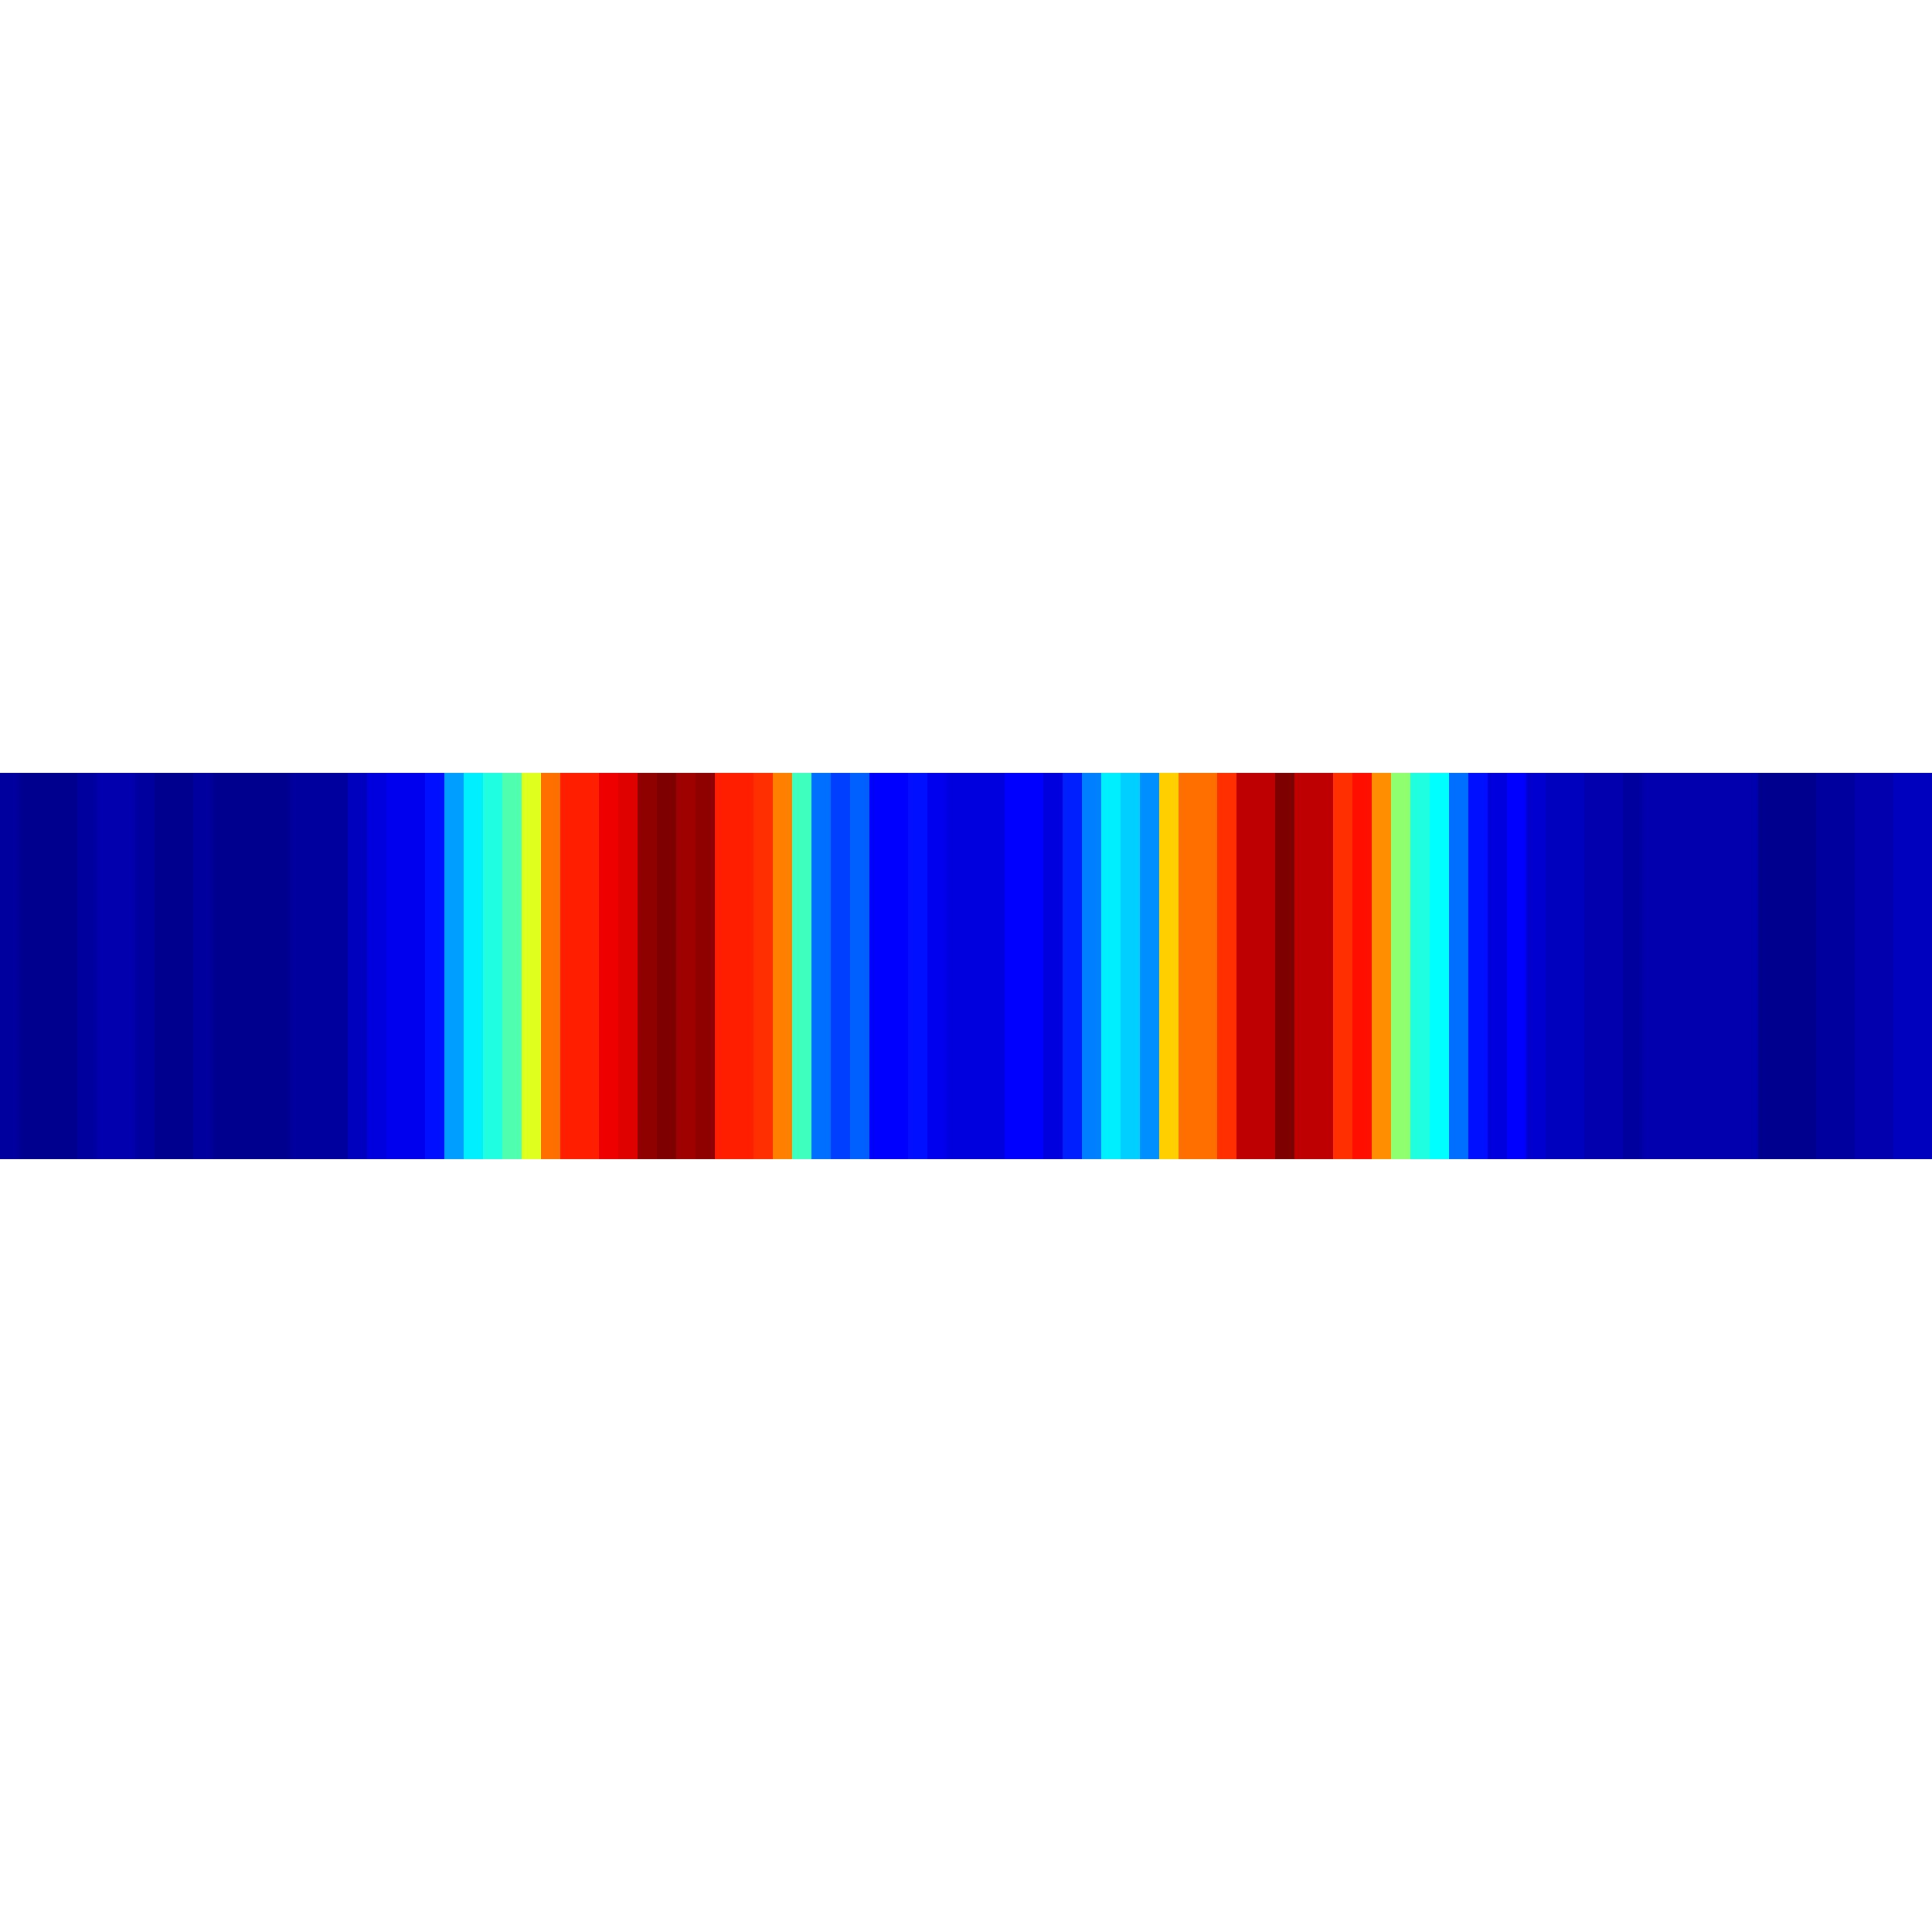
\includegraphics[width=0.2\textwidth, height=0.1in]{line_profile.jpg}} edge[<-] (dpERK_circle);
		\node [below=0in of dpERK_line, text width=0.2\textwidth, align=center] (text1) {{\scriptsize The circumference of the embryo is ``unrolled'' to form an intensity profile for the embryo on a line \par}};
		
	\end{tikzpicture}
	
	\centering
    \begin{tikzpicture}
        \node (fig1) {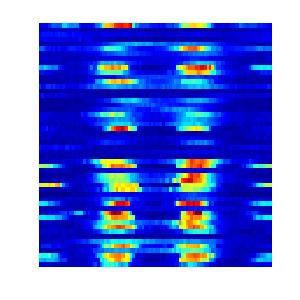
\includegraphics[width=0.35\textwidth]{data_unordered}};
        \node[right of=fig1, node distance=0.55\textwidth] (fig2) {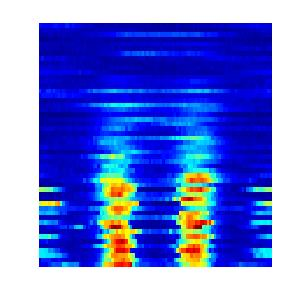
\includegraphics[width=0.35\textwidth]{data_ordered_membrane}};
        \draw [->] (fig1.east) -- (fig2.west) node[above,midway] {\tiny Order using membrane thickness};
    \end{tikzpicture}
	
	We would like to order the snapshots {\em without} measuring the membrane thickness.
	
\end{frame}
